
\documentclass[11pt]{article}
\usepackage[paper=letterpaper, margin=.5in]{geometry}
\pdfpagewidth 8.5in
\pdfpageheight 11in
\setlength\parindent{0in}

%% AMS PACKAGES - Chances are you will want some or all of these if writing a math dissertation.
\usepackage{amsmath, amscd, amssymb, amsthm, multirow, enumerate, multicol, graphicx, listings, placeins}
\newcommand{\Z}{\mathbb{Z}}
\newcommand{\R}{\mathbb{R}}
\newcommand{\Q}{\mathbb{Q}}
\newcommand{\C}{\mathbb{C}}
\newcommand{\N}{\mathbb{N}}
\newcommand{\V}{\mathbb{V}}
\newcommand{\U}{\mathcal{U}}
\newcommand{\del}{\partial}
\newcommand{\real}{\textrm{Re }}
\newcommand{\imag}{\textrm{Im }}
\newcommand{\pd}[2]{\frac{\partial #1}{\partial #2}}
\newcommand{\deriv}[2]{\frac{d #1}{d #2}}
\newcommand{\sumk}{\sum_{k=1}^\infty}
\newcommand{\sumj}{\sum_{j=1}^\infty}
\newcommand{\sumn}{\sum_{n=0}^\infty}
\newcommand{\summ}[2]{\sum_{k=#1}^{#2}}
\newcommand{\sig}[1]{\sum_{#1 =1}^\infty}
\newcommand{\un}[1]{\bigcup_{#1 =1}^\infty}
\newcommand{\inter}[1]{\bigcap_{#1 =1}^\infty}
\newcommand{\ip}[2]{\langle #1, #2 \rangle}
\newcommand{\ipxu}{\langle x,u_j \rangle}
\newcommand{\uj}{\{u_j\}_{j=1}^\infty}
\newcommand{\B}{\mathcal{B}}

\newcommand{\E}{\mathrm{E}}
\newcommand{\var}{\mathrm{Var}}
\newcommand{\cov}{\mathrm{Cov}}
\newcommand{\ST}{mbox{ s.t. }}

\newcommand{\Example}{\noindent {\bf Example. \quad} }
\newcommand{\Proof}{\noindent {\bf Proof: \quad} }
\newcommand{\Remark}{\noindent {\bf Remark. \quad} }
\newcommand{\Remarks}{\noindent {\bf Remarks. \quad} }
\newcommand{\Case}{\noindent {\underline{Case} \quad} }

\newcommand{\st}{ \; \big | \:}

\newcommand{\deuc}{d_{\mathrm euc}}
\newcommand{\dtaxi}{d_{\mathrm taxi}}
\newcommand{\ddisc}{d_{\mathrm disc}}
\newtheorem{theorem}{Theorem}[section]
\newtheorem{lemma}[theorem]{Lemma}
\newtheorem{proposition}[theorem]{Proposition}
\newtheorem{corollary}[theorem]{Corollary}
\theoremstyle{definition}
\newtheorem{definition}[theorem]{Definition}
\newtheorem{example}[theorem]{Example}

\begin{document}
%%%%%%%%%%%%%%%%%%%%%%%%%%%%%%%%%%%%%%%%%%%%%%%%%%%%%%%%%%%%%%%%%%%%%%%%%%%%%%%%%%%%%%%%%%%%%%%%%%%%%%%%%%%%%%%%%%%%%%%%%%%%%%%%%%%%%
STAT 343, Homework 6 \hfill Aaron Maurer
\vspace{2mm}
\hrule
\vspace{2mm}
\begin{itemize}
    \item[1.] Problem 5.3 in Weisberg \\
        I got an estimate of \(\hat\sigma^2=1860.276\), so for the test statistic I got that \(G=\frac{\sum_{i=1}^n(\hat y_i - \tilde y_i)^2}{\hat\sigma^2}=15.296\). Then, running the bootstrap algorithm with $1000$ bootstraps, I got a significance level of  $.002$, since only $\frac{1}{1000}$ of the bootstrap samples resulted in a higher test statistic.
    \item[2.]
        \begin{itemize}
            \item[a)]
                \begin{align*}
                    X_{(i)}^TX_{(i)}&=\sum_{j\neq i} x_j^Tx_j \\
                    X_{(i)}^TX_{(i)}&= X^TX - x_i^Tx_i \\
                    (X_{(i)}^TX_{(i)})^{-1}&= (X^TX - x_i^Tx_i)^{-1} \\
                \end{align*}
                Applying the Sherman-Morrison formula to the right hand side, we get
                \begin{align*}
                    (X_{(i)}^TX_{(i)})^{-1}&= (X^TX)^{-1} + \frac{(X^TX)^{-1}x_i^Tx_i(X^TX)^{-1}}{1-x_i(X^TX)^{-1}x_i^T} \\
                    (X_{(i)}^TX_{(i)})^{-1}&= (X^TX)^{-1} + \frac{(X^TX)^{-1}x_i^Tx_i(X^TX)^{-1}}{1-h_{ii}} \\
                \end{align*}
            \item[b)]
                \begin{align*}
                    \hat \beta_{(i)} &= (X_{(i)}^TX_{(i)})^{-1}X_{(i)}^T Y_{(i)}   \\
                    \hat \beta_{(i)} &= \left((X^TX)^{-1} + \frac{(X^TX)^{-1}x_i^Tx_i(X^TX)^{-1}}{1-h_{ii}} \right)\left(X^TY - x_i^Ty_i\right)  \\
                    \hat \beta_{(i)} &= (X^TX)^{-1}\left(X^TY - x_i^Ty_i\right) + \frac{(X^TX)^{-1}x_i^Tx_i(X^TX)^{-1}}{1-h_{ii}}\left(X^TY - x_i^T y_i\right)   \\
                    \hat \beta_{(i)} &= \hat \beta - (X^TX)^{-1}x_i^Ty_i + \frac{(X^TX)^{-1}x_i^Tx_i(X^TX)^{-1}\left(X^TY - x_i^T y_i\right)}{1-h_{ii}}   \\
                    \hat \beta_{(i)} &= \hat \beta + \frac{(X^TX)^{-1}x_i^Ty_i(h_{ii}-1) +(X^TX)^{-1}x_i^T\left(x_i\hat\beta - h_{ii}y_i\right)}{1-h_{ii}}   \\
                    \hat \beta_{(i)} &= \hat \beta + \frac{(X^TX)^{-1}x_i^T\left(x_i\hat\beta - h_{ii}y_i + (h_{ii}-1)y_i\right)}{1-h_{ii}}   \\
                    \hat \beta_{(i)} &= \hat \beta + \frac{(X^TX)^{-1}x_i^T\left(x_i\hat\beta - y_i\right)}{1-h_{ii}} \\
                    \hat \beta_{(i)} &= \hat \beta - \frac{(X^TX)^{-1}x_i^T\hat e_i}{1-h_{ii}}   
                \end{align*}
            \item[c)]
                \begin{align*}
                    y_i - x_i\hat\beta_{(i)} &= y_i- x_i\left(\hat \beta - \frac{(X^TX)^{-1}x_i^T\hat e_i}{1-h_{ii}}\right) \\
                    y_i - x_i\hat\beta_{(i)} &= y_i  - \hat y_i + \frac{h_{ii}\hat e_i}{1-h_{ii}} \\
                    y_i - x_i\hat\beta_{(i)} &= \hat e_i \left(1+ \frac{h_{ii}}{1-h_{ii}}\right) \\
                    y_i - x_i\hat\beta_{(i)} &= \hat e_i \frac{1}{1-h_{ii}} \\
                \end{align*}
            \item[d)]
                \begin{align*}
                    D_i &= \frac{\|\hat Y_{(i)} - \hat Y\|^2}{p\hat\sigma^2} \\
                    D_i &= \frac{\|X\beta_{(i)} - X\beta\|^2}{p\hat\sigma^2} \\
                    D_i &= \frac{\|X\left(\hat \beta - \frac{(X^TX)^{-1}x_i^T\hat e_i}{1-h_{ii}}\right) - X\beta\|^2}{p\hat\sigma^2} \\
                    D_i &= \frac{\|- X\frac{(X^TX)^{-1}x_i^T\hat e_i}{1-h_{ii}}\|^2}{p\hat\sigma^2} \\
                    D_i &= \frac{\frac{\hat e_ix_i(X^TX)^{-1}}{1-h_{ii}}X^TX\frac{(X^TX)^{-1}x_i^T\hat e_i}{1-h_{ii}}}{p\hat\sigma^2} \\
                    D_i &= \frac{\frac{\hat e_ix_i(X^TX)^{-1}}{1-h_{ii}}X^TX\frac{(X^TX)^{-1}x_i^T\hat e_i}{1-h_{ii}}}{p\hat\sigma^2} \\
                    D_i &= \frac{\frac{\hat e_ix_i(X^TX)^{-1}}{1-h_{ii}}\frac{x_i^T\hat e_i}{1-h_{ii}}}{p\hat\sigma^2} \\
                    D_i &= \frac{1}{p}\frac{\hat e_i^2}{\hat\sigma^2(1-h_{ii})}\frac{x_i(X^TX)^{-1}x_i^T}{1-h_{ii}} \\
                    D_i &= \frac{1}{p} r_i^2 \frac{h_ii}{1-h_{ii}} 
                \end{align*}
        \end{itemize}
    \item[3)]
        \begin{itemize}
            \item[a)]
                The two graphs make it pretty clear there is autocorrelated errors. The first, ``Residual by Year", seems to show the errors moving up and down together, rather than being the cloud centered around $0$ if there was no autocorrelation. The second, ``Residual vs Residual With Lag of 1" shows each residual plotted against the next residual. The evidence of autocorrelation is overwhelming here, with there being a clear positive linear relationship between one error and the next. \\
                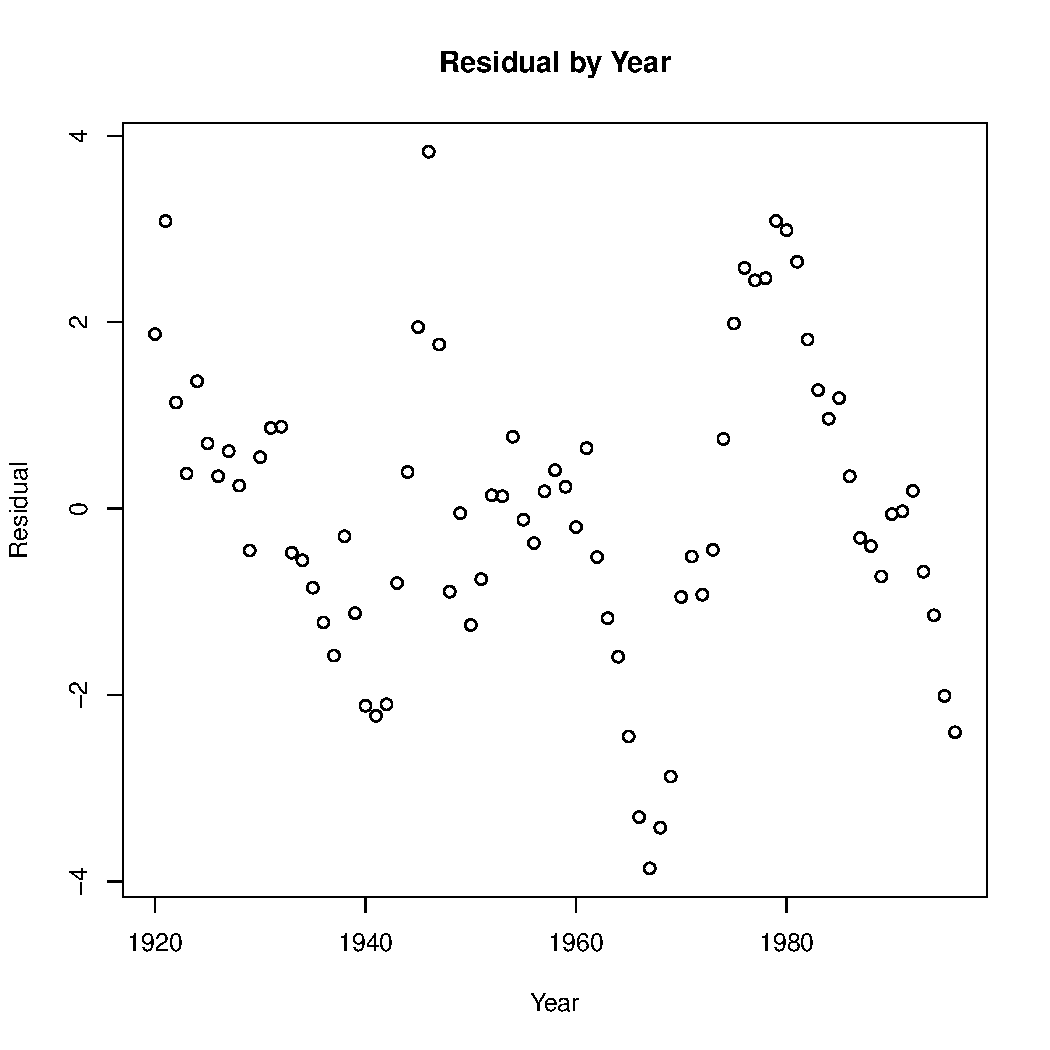
\includegraphics[width=9cm]{hw6_3_a_res} 
                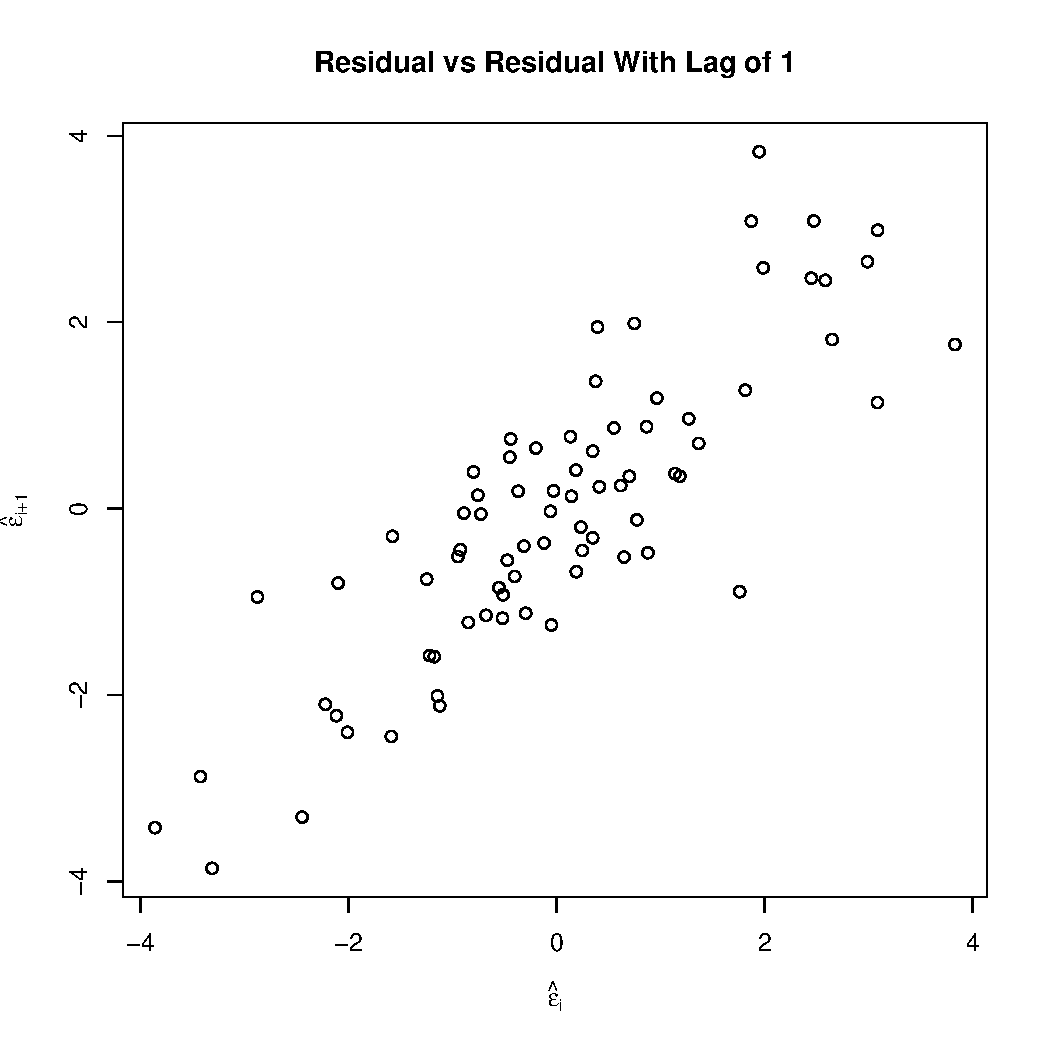
\includegraphics[width=9cm]{hw6_3_a_auto}  \\
            \item[b)]
                Running the AR1 model, we see an estimated autocorrelation of $.972$, which is extremely significant. We also see unemployed switch to being significant with a p-value of $.02$ in the AR1 model while just outside of of significance at $.051$ in the ordinary linear model. Much more importantly though, the coefficient switches sign, speaking to the autocorrelation having a meaningful effect.\\
                Confidence interval and estimate for autocorrelation: \\
                \FloatBarrier
                % latex table generated in R 3.1.1 by xtable 1.7-4 package
% Wed Nov 19 11:57:19 2014
\begin{table}[ht]
\centering
\begin{tabular}{rrrr}
  \hline
 & lower & est. & upper \\ 
  \hline
Phi & 0.653 & 0.972 & 0.998 \\ 
   \hline
\end{tabular}
\end{table}
 
                \FloatBarrier

                Coefficients for autocorrelated model: \\
                \FloatBarrier
                % latex table generated in R 3.1.1 by xtable 1.7-4 package
% Wed Nov 19 11:57:19 2014
\begin{table}[ht]
\centering
\begin{tabular}{rrrrr}
  \hline
 & Value & Std.Error & t-value & p-value \\ 
  \hline
(Intercept) & -7.060 & 5.547 & -1.273 & 0.207 \\ 
  unemployed & 0.108 & 0.046 & 2.344 & 0.022 \\ 
  femlab & 0.312 & 0.095 & 3.280 & 0.002 \\ 
  marriage & 0.164 & 0.023 & 7.177 & 0.000 \\ 
  birth & -0.050 & 0.022 & -2.267 & 0.026 \\ 
  military & 0.018 & 0.014 & 1.258 & 0.213 \\ 
   \hline
\end{tabular}
\end{table}

                \FloatBarrier

                Coefficients for regular linear model: \\
                \FloatBarrier
                % latex table generated in R 3.1.1 by xtable 1.7-4 package
% Wed Nov 19 11:57:19 2014
\begin{table}[ht]
\centering
\begin{tabular}{rrrrr}
  \hline
 & Estimate & Std. Error & t value & Pr($>$$|$t$|$) \\ 
  \hline
(Intercept) & 2.488 & 3.394 & 0.733 & 0.466 \\ 
  unemployed & -0.111 & 0.056 & -1.989 & 0.051 \\ 
  femlab & 0.384 & 0.031 & 12.543 & 0.000 \\ 
  marriage & 0.119 & 0.024 & 4.861 & 0.000 \\ 
  birth & -0.130 & 0.016 & -8.333 & 0.000 \\ 
  military & -0.027 & 0.014 & -1.876 & 0.065 \\ 
   \hline
\end{tabular}
\end{table}

                \FloatBarrier

                Only one coefficient, that of unemployed, switched to the other side of the $.05$ threshold with the auto correlated term, but the estimate and p-value of all the other variables changes noticeably, speaking to how not dealing with autocorrelation can invalidate a model.

            \item[c)]
                My suspicion is that the autocorrelation largely has to do with the relative size of different generations. The portion of the US population in different age groups varies a lot over time, and divorce rates are likely quite different between different age groups. Since the relative portion of people in each age group is highly auto-correlated (since everyone either dies or gets just one year older), our divorce rate is also auto-correlated.
        \end{itemize}
    \item[4)]
        It looks like we have a lack of fit since the variance isn't constant. Looking at the first plot, the residual plot, nothing is glaringly wrong, but it looks like the points farther to the right are somewhat more spread out. Plotting the square root transformed residuals against the predicted values, and adding a trend line, we see a much more obvious increase in variance over the range, with a clear upwards trend. Testing this formally with the variance test, where we split the residuals into those with speed above and below 14, we get a ratio of $.206$, with an associated p-value of $.0009$, which seals it. We also appear to have a mildly non-linear response. \\
        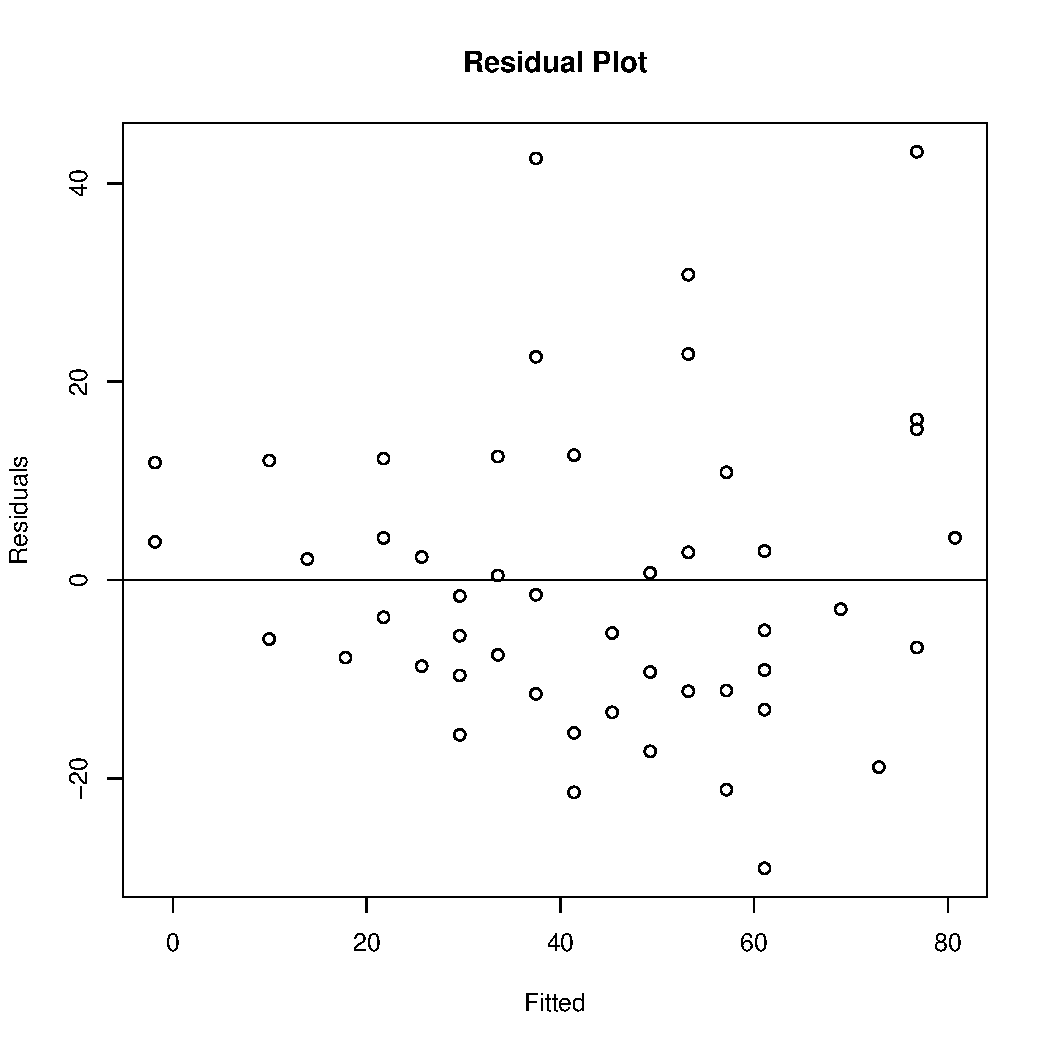
\includegraphics[width=9cm]{hw6_4_res} 
        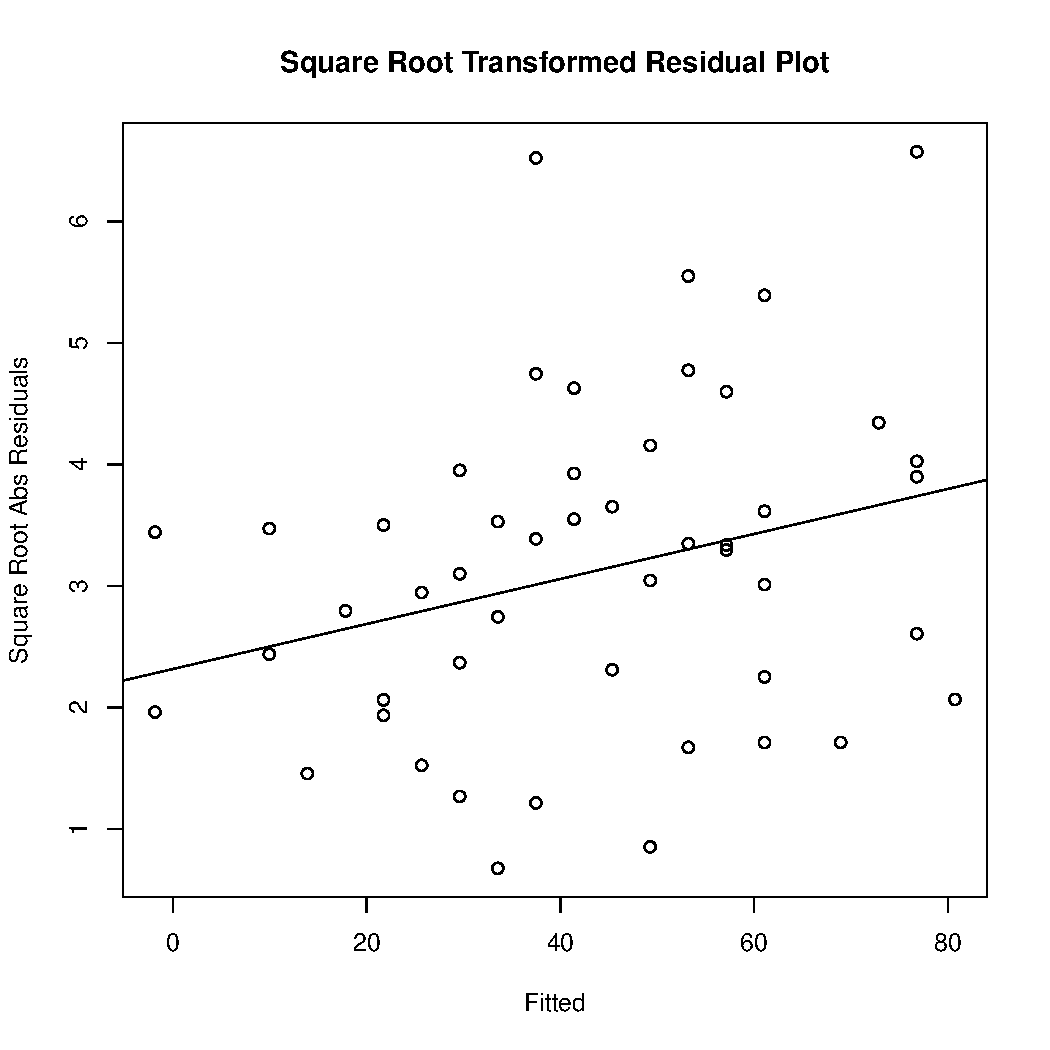
\includegraphics[width=9cm]{hw6_4_sqrtres}  \\
             As far as other issues, none jump out. From the residual plot, no residual looks extreme enough to be an outlier. Running a QQ plot, the residuals on the whole look roughly normal. \\
        \begin{center}
            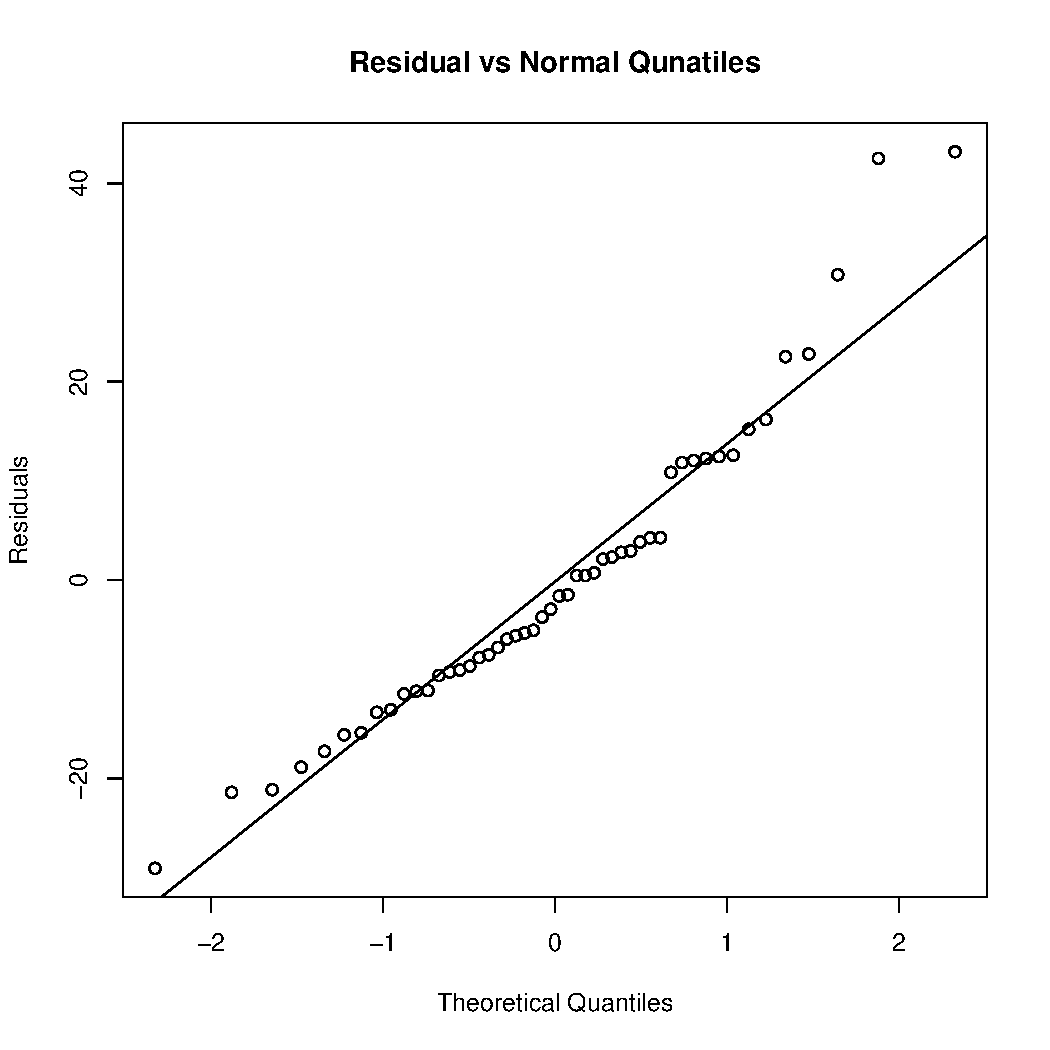
\includegraphics[width=9cm]{hw6_4_qq} 
        \end{center}
        The one potential issue is that the true relationship between the predictor and outcome may not quite be linear. Looking at the linear fit versus a kernel regression fit, it seems like the function may actual be somewhat convex. 
        \begin{center}
            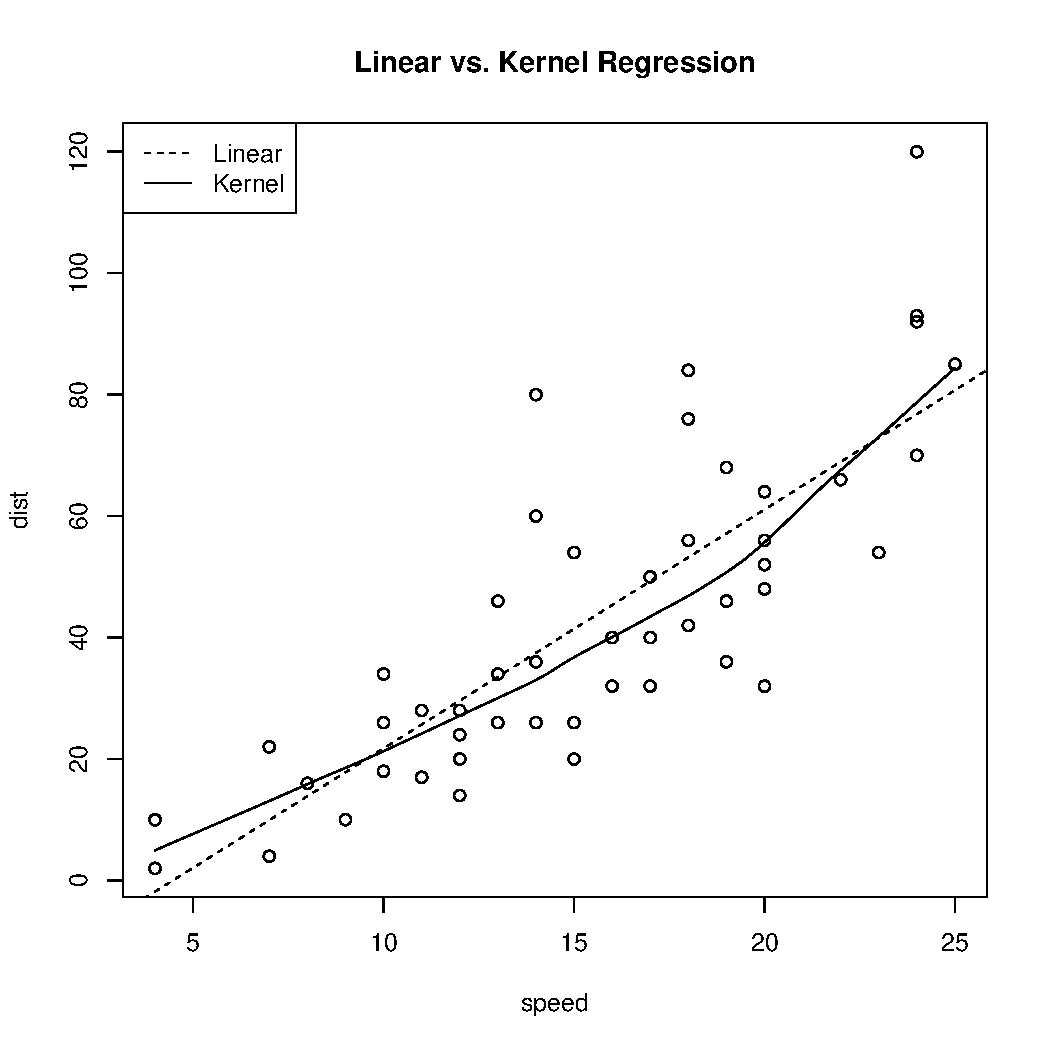
\includegraphics[width=9cm]{hw6_4_ker} 
        \end{center}
        Attempting to approximate this with a linear spline, we allow for a different slope above and below a speed of $20$, where we seem to have a mild kink. When we do this, and run we ANOVA, we just get significant decrease in variance, with a p-value of $.0378$. \\
        % latex table generated in R 3.1.1 by xtable 1.7-4 package
% Wed Nov 19 11:57:19 2014
\begin{table}[ht]
\centering
\begin{tabular}{lrrrrrr}
  \hline
 & Res.Df & RSS & Df & Sum of Sq & F & Pr($>$F) \\ 
  \hline
1 & 48.000 & 11353.521 &  &  &  &  \\ 
  2 & 47.000 & 10347.643 & 1.000 & 1005.878 & 4.569 & 0.038 \\ 
   \hline
\end{tabular}
\end{table}

    \item[5)]
        In general, it seems to be the case that without dealing with outliers, one can get meaningfully different results between robust regression and non-robust regression. However, when outliers are taken out, they give much more similar results. We see this most strongly with the coefficient for air flow. With the outlier in, we get coefficients of about $.8$ with robust regression and a smaller, though still significant, coefficient of $.7$ with regular linear regression. When an outlier is removed, all the methods get about $.8$.\\

        \smallskip
        With the outliers in, we got the results below. In addition to the difference with air flow noted above, the coefficient with water temp seems to vary a lot between methods, though is always significant, while  acid concentration is significant in every one except the least absolute deviation, where its just barely significant.
        \begin{itemize}
            \item[a)] Regular least squares: \\
                \FloatBarrier
                % latex table generated in R 3.1.1 by xtable 1.7-4 package
% Wed Nov 19 11:57:19 2014
\begin{table}[ht]
\centering
\begin{tabular}{rrrrr}
  \hline
 & Estimate & Std. Error & t value & Pr($>$$|$t$|$) \\ 
  \hline
(Intercept) & -39.920 & 11.896 & -3.356 & 0.004 \\ 
  Acid.Conc. & -0.152 & 0.156 & -0.973 & 0.344 \\ 
  Water.Temp & 1.295 & 0.368 & 3.520 & 0.003 \\ 
  Air.Flow & 0.716 & 0.135 & 5.307 & 0.000 \\ 
   \hline
\end{tabular}
\end{table}

                \FloatBarrier
            \item[b)] Least absolute deviation: \\
                \FloatBarrier
                % latex table generated in R 3.1.1 by xtable 1.7-4 package
% Wed Nov 19 11:57:19 2014
\begin{table}[ht]
\centering
\begin{tabular}{rrrr}
  \hline
 & coefficients & lower bd & upper bd \\ 
  \hline
(Intercept) & -39.690 & -41.620 & -29.678 \\ 
  Acid.Conc. & -0.061 & -0.213 & -0.029 \\ 
  Water.Temp & 0.574 & 0.322 & 1.411 \\ 
  Air.Flow & 0.832 & 0.523 & 1.141 \\ 
   \hline
\end{tabular}
\end{table}

                \FloatBarrier
            \item[c)] Hubber method:\\
                \FloatBarrier
                % latex table generated in R 3.1.1 by xtable 1.7-4 package
% Wed Nov 19 11:57:19 2014
\begin{table}[ht]
\centering
\begin{tabular}{rrrr}
  \hline
 & Value & Std. Error & t value \\ 
  \hline
(Intercept) & -41.027 & 9.807 & -4.183 \\ 
  Acid.Conc. & -0.128 & 0.129 & -0.992 \\ 
  Water.Temp & 0.926 & 0.303 & 3.052 \\ 
  Air.Flow & 0.829 & 0.111 & 7.460 \\ 
   \hline
\end{tabular}
\end{table}

                \FloatBarrier
            \item[d)] Least trimmed squares: \\
                \FloatBarrier
                % latex table generated in R 3.1.1 by xtable 1.7-4 package
% Wed Nov 19 11:57:19 2014
\begin{table}[ht]
\centering
\begin{tabular}{rr}
  \hline
 & coef(sl.lts) \\ 
  \hline
(Intercept) & -35.806 \\ 
  Acid.Conc. & -0.000 \\ 
  Water.Temp & 0.333 \\ 
  Air.Flow & 0.750 \\ 
   \hline
\end{tabular}
\end{table}

                \FloatBarrier
        \end{itemize}
        Looking at the Cook's Distances, its clear that the $21$st observation is immensely influential. $3$, $4$, and $1$ also have relatively high Cook's Distances, but they don't seem that out of line with the rest of them. Double checking the studentized residuals, $21$ a value of $3.330$, while the next highest is $2.052$. Since the Bonferroni critical value at a p-value of $.05$ is $3.256$, I concluded that $21$ is worth removing, while the rest can remain.
        \begin{center}
            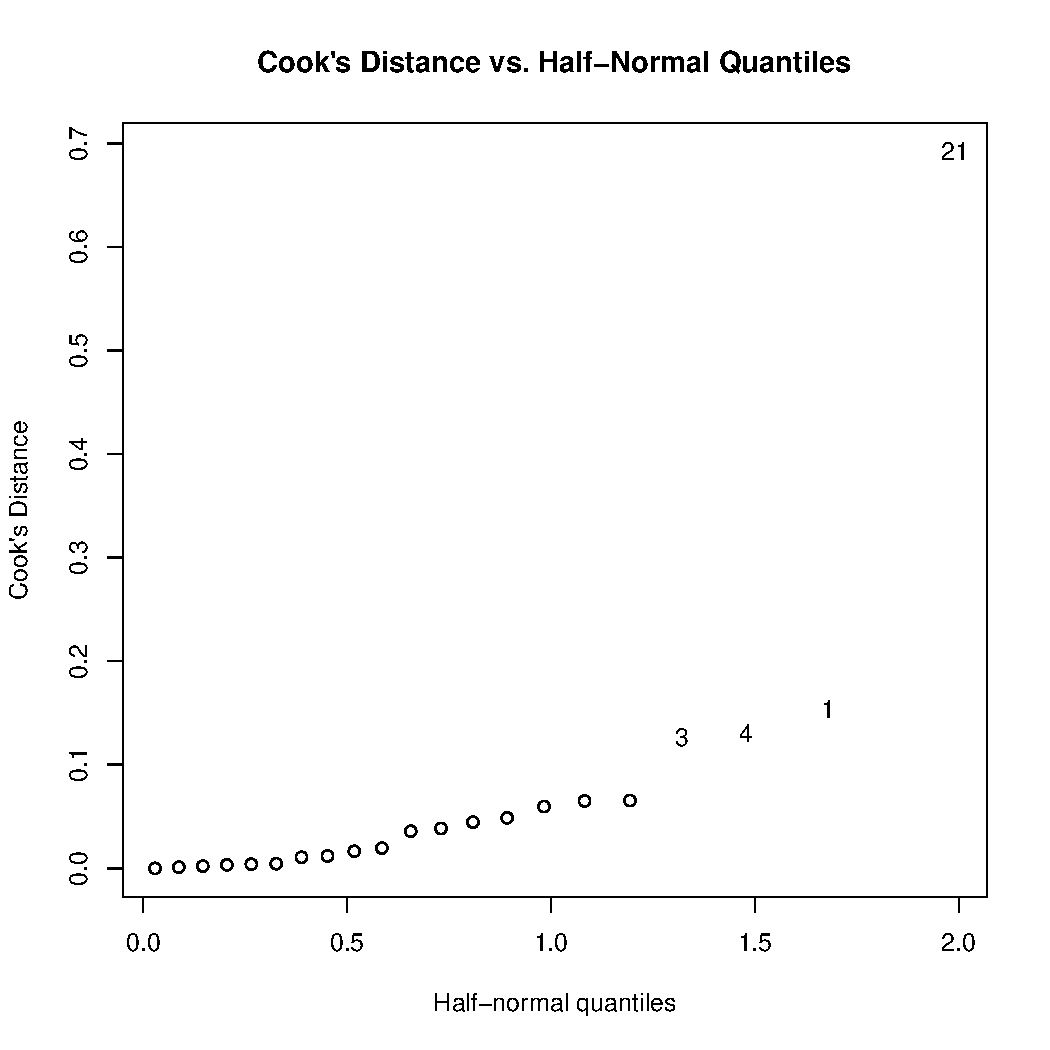
\includegraphics[width=9cm]{hw6_5_halfnorm} 
        \end{center}
        Looking over the effects of the inclusion of each observation on the coefficients, we see that $21$ has a much bigger effect over air flow and water temp than other variables, further supporting that it should be removed as an outlier. \\ 
            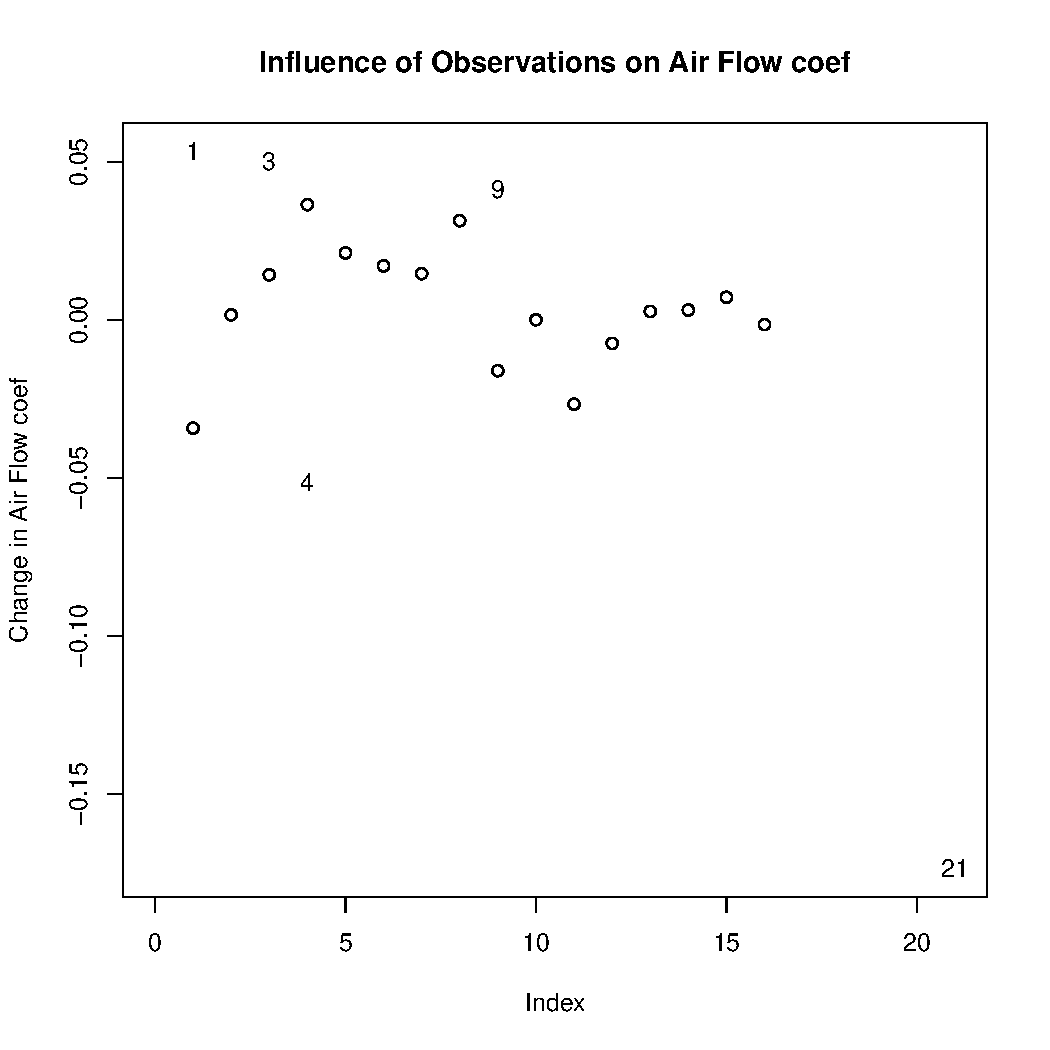
\includegraphics[width=9cm]{hw6_5_af} 
            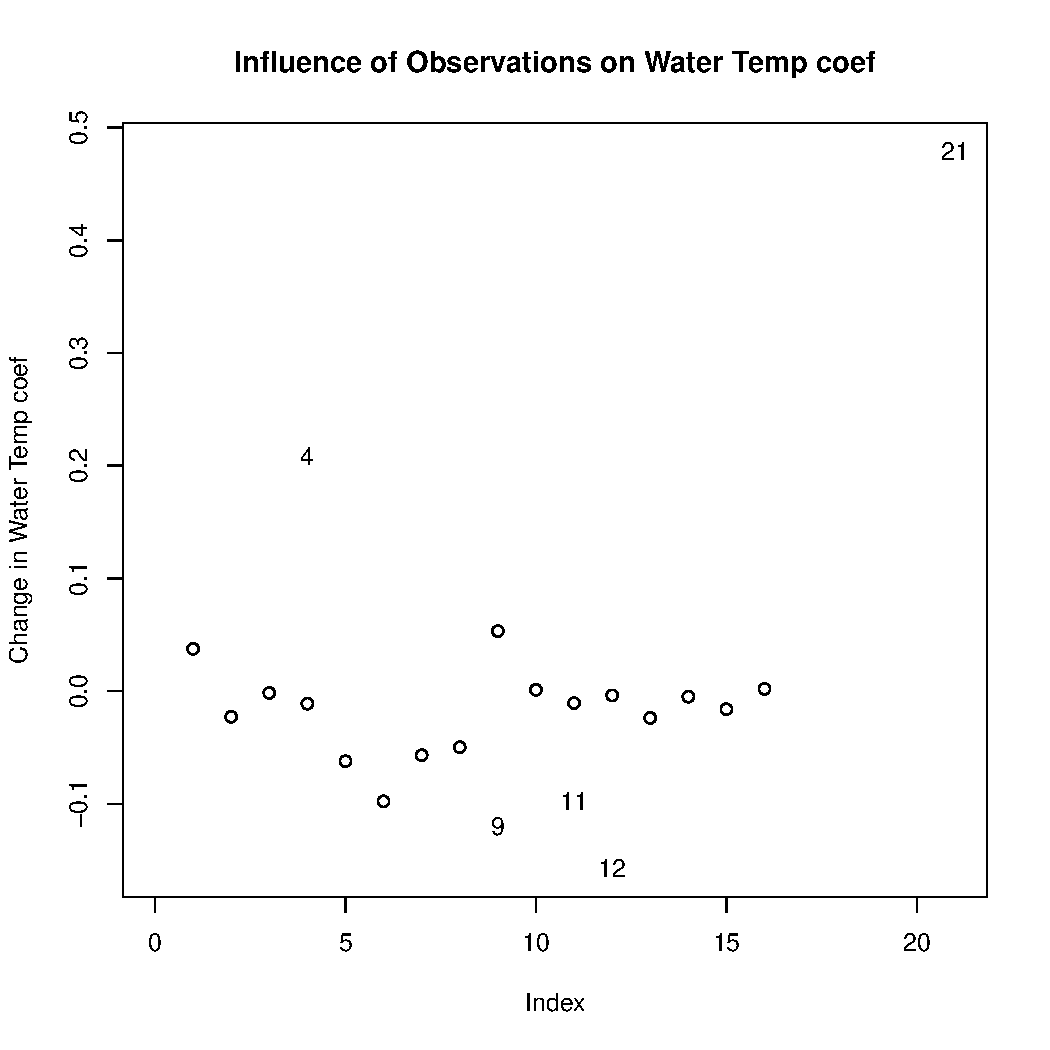
\includegraphics[width=9cm]{hw6_5_wt} \\

        Rerunning each of the regressions with $21$ removed, we get the results below. The air flow coefficient is now fairly consistent between the robust and non-robust regressions. The water temp coefficient is still meaningfully different between the robust and non-robust regressions, though much smaller than before. It may be that observation $4$, as seen above, is still having undue influence. Finally, acid concentration continues to be insignificant, or just barely significant.
        \begin{itemize}
            \item[a)] Regular least squares: \\
                \FloatBarrier
                % latex table generated in R 3.1.1 by xtable 1.7-4 package
% Wed Nov 19 11:57:19 2014
\begin{table}[ht]
\centering
\begin{tabular}{rrrrr}
  \hline
 & Estimate & Std. Error & t value & Pr($>$$|$t$|$) \\ 
  \hline
(Intercept) & -43.704 & 9.492 & -4.605 & 0.000 \\ 
  Acid.Conc. & -0.107 & 0.125 & -0.860 & 0.402 \\ 
  Water.Temp & 0.817 & 0.325 & 2.512 & 0.023 \\ 
  Air.Flow & 0.889 & 0.119 & 7.481 & 0.000 \\ 
   \hline
\end{tabular}
\end{table}

                \FloatBarrier
            \item[b)] Least absolute deviation: \\
                \FloatBarrier
                % latex table generated in R 3.1.1 by xtable 1.7-4 package
% Wed Nov 19 11:57:19 2014
\begin{table}[ht]
\centering
\begin{tabular}{rrrr}
  \hline
 & coefficients & lower bd & upper bd \\ 
  \hline
(Intercept) & -39.986 & -54.137 & -30.213 \\ 
  Acid.Conc. & -0.057 & -0.398 & -0.035 \\ 
  Water.Temp & 0.564 & 0.267 & 1.107 \\ 
  Air.Flow & 0.835 & 0.825 & 1.167 \\ 
   \hline
\end{tabular}
\end{table}

                \FloatBarrier
            \item[c)] Hubber method:\\
                \FloatBarrier
                % latex table generated in R 3.1.1 by xtable 1.7-4 package
% Wed Nov 19 11:57:19 2014
\begin{table}[ht]
\centering
\begin{tabular}{rrrr}
  \hline
 & Value & Std. Error & t value \\ 
  \hline
(Intercept) & -42.841 & 8.619 & -4.970 \\ 
  Acid.Conc. & -0.108 & 0.113 & -0.953 \\ 
  Water.Temp & 0.685 & 0.295 & 2.322 \\ 
  Air.Flow & 0.918 & 0.108 & 8.509 \\ 
   \hline
\end{tabular}
\end{table}

                \FloatBarrier
            \item[d)] Least trimmed squares: \\
                \FloatBarrier
                % latex table generated in R 3.1.1 by xtable 1.7-4 package
% Wed Nov 19 11:57:19 2014
\begin{table}[ht]
\centering
\begin{tabular}{rr}
  \hline
 & coef(sl.lts.no) \\ 
  \hline
(Intercept) & -35.806 \\ 
  Acid.Conc. & -0.000 \\ 
  Water.Temp & 0.333 \\ 
  Air.Flow & 0.750 \\ 
   \hline
\end{tabular}
\end{table}

                \FloatBarrier
        \end{itemize}

    
\end{itemize}

\end{document}
